\documentclass{article}

% content/resources/templates/preamble.tex
\usepackage[margin=0.6in]{geometry}
\author{Milav Dabgar}
\usepackage{amsmath,amssymb,amsthm}
\usepackage{booktabs}
\usepackage{multirow}
\usepackage{xcolor}
\usepackage{tcolorbox}
\tcbuselibrary{breakable,skins}
\usepackage[colorlinks=true,linkcolor=blue]{hyperref}
\usepackage{titlesec}
\usepackage{enumitem}
\usepackage{tikz}
\usepackage{pgfplots}
\usepackage{circuitikz}
\usepackage[version=4]{mhchem}
\usepackage{longtable}
\usepackage{array}
\usepackage{float}
\usepackage{caption}
\usepackage{listings}

\lstset{
  basicstyle=\small\ttfamily,
  breaklines=true,
  breakatwhitespace=false,
  postbreak=\mbox{\textcolor{red}{$\hookrightarrow$}\space},
  float=false,
  numbers=left,
  numberstyle=\tiny\color{gray},
  numbersep=10pt,
  xleftmargin=2em,
  keywordstyle=\color{blue},
  commentstyle=\color{green!60!black},
  stringstyle=\color{purple},
  backgroundcolor=\color{gray!5},
  showstringspaces=false,
  tabsize=2,
  captionpos=b,
  keepspaces=true,
  columns=flexible
}

\pgfplotsset{compat=1.18}
\usetikzlibrary{shapes,arrows,positioning,calc,patterns,decorations.pathmorphing,decorations.markings,arrows.meta}

% Color scheme
\definecolor{headcolor}{RGB}{0,102,204}
\definecolor{keycolor}{RGB}{220,20,60}
\definecolor{solutioncolor}{RGB}{34,139,34}
\definecolor{mnemoniccolor}{RGB}{148,0,211}
\definecolor{codecolor}{RGB}{0,0,100}

% Spacing
\setlength{\parskip}{3pt}
\setlist[itemize]{nosep}
\setlist[enumerate]{nosep}

% Title formatting
\titleformat{\section}{\Large\bfseries\color{headcolor}}{\thesection}{1em}{}
\titleformat{\subsection}{\large\bfseries\color{headcolor}}{\thesubsection}{1em}{}

% Pandoc tightlist compatibility
\providecommand{\tightlist}{%
  \setlength{\itemsep}{0pt}\setlength{\parskip}{0pt}}

% Pandoc longtable compatibility
\newcounter{none}
\def\thenone{}


% content/resources/templates/english-boxes.tex

% Custom environments
\newtcolorbox{solutionbox}{
 breakable,
 enhanced,
 colback=solutioncolor!5!white,
 colframe=solutioncolor!75!black,
 fonttitle=\bfseries,
 title=Solution
}

\newtcolorbox{solutionboxnobreak}{
 colback=solutioncolor!5!white,
 colframe=solutioncolor!75!black,
 fonttitle=\bfseries,
 title=Solution
}

\newtcolorbox{keyformula}{
 breakable,
 enhanced,
 colback=keycolor!5!white,
 colframe=keycolor!75!black,
 fonttitle=\bfseries,
 title=Key Formula
}

\newtcolorbox{mnemonicboxenv}{
 breakable,
 enhanced,
 colback=mnemoniccolor!5!white,
 colframe=mnemoniccolor!75!black,
 fonttitle=\bfseries,
 title=Mnemonic
}

\newcommand{\mnemonicbox}[1]{%
  \begin{mnemonicboxenv}
    #1
  \end{mnemonicboxenv}
}


% Custom commands for GTU solutions
% This file defines semantic commands for consistent formatting

% Question command with automatic formatting
\newcommand{\question}[2]{%
  \section*{Question #1}%
  \textbf{#2}%
}

% OR question variant
\newcommand{\questionor}[2]{%
  \section*{Question #1 OR}%
  \textbf{#2}%
}

% Proper table environment with caption
\newenvironment{answertable}[1]{%
  \begin{table}[htbp]
  \centering
  \caption{#1}
}{%
  \end{table}
}

% Proper figure environment for diagrams
\newenvironment{answerdiagram}[1]{%
  \begin{figure}[htbp]
  \centering
  \caption{#1}
}{%
  \end{figure}
}

% Semantic markup for key terms
\newcommand{\keyword}[1]{\textbf{#1}}
\newcommand{\code}[1]{\texttt{#1}}
\newcommand{\classname}[1]{\texttt{#1}}
\newcommand{\methodname}[1]{\texttt{#1}}

% Proper quotation marks
\newcommand{\mnemonic}[1]{``#1''}


\title{Environment and Sustainability (4300003) - Winter 2021 Solution}
\date{March 24, 2022}

\begin{document}
\maketitle

\questionmarks{1}{}{14}
\textbf{Answer any seven questions.}

\subsubsection{1. Define the terms: 'Ecology' and 'Ecosystem'.}

\begin{solutionbox}
    \textbf{Definitions:}
    \textbf{Ecology} is the scientific study of relationships between living organisms and their environment. \textbf{Ecosystem} is a biological community of interacting organisms and their physical environment functioning as a unit.

    \begin{answertable}{Terms and Definitions}
    \begin{tabulary}{\linewidth}{L L L}
        \toprule
        \textbf{Term} & \textbf{Definition} & \textbf{Example} \\
        \midrule
        \textbf{Ecology} & Study of organism-environment relationships & Forest ecology \\
        \textbf{Ecosystem} & Living and non-living components interaction & Pond ecosystem \\
        \bottomrule
    \end{tabulary}
    \end{answertable}

    \begin{itemize}
        \item \textbf{Biotic components}: Living organisms in the system
        \item \textbf{Abiotic components}: Non-living factors like air, water, soil
    \end{itemize}

    \begin{mnemonicbox}Every Component Lives Together (Ecology Creates Living Together)\end{mnemonicbox}
\end{solutionbox}

\subsubsection{2. Define the terms: 'Pollution' and 'Pollutant'.}

\begin{solutionbox}
    \textbf{Definitions:}
    \textbf{Pollution} is the introduction of harmful substances into the environment causing adverse effects. \textbf{Pollutant} is any substance that causes pollution when present in excessive amounts.

    \begin{answertable}{Pollution Terms}
    \begin{tabulary}{\linewidth}{L L L}
        \toprule
        \textbf{Term} & \textbf{Definition} & \textbf{Types} \\
        \midrule
        \textbf{Pollution} & Environmental contamination & Air, Water, Soil, Noise \\
        \textbf{Pollutant} & Harmful substance & Physical, Chemical, Biological \\
        \bottomrule
    \end{tabulary}
    \end{answertable}

    \begin{itemize}
        \item \textbf{Primary pollutants}: Directly emitted substances
        \item \textbf{Secondary pollutants}: Formed by reactions in atmosphere
    \end{itemize}

    \begin{mnemonicbox}Pollution Produces Problems (Pollutants Produce Problems)\end{mnemonicbox}
\end{solutionbox}

\subsubsection{3. What is noise pollution? What is unit of intensity of sound?}

\begin{solutionbox}
    \textbf{Noise pollution} is unwanted or excessive sound that disrupts human activities and harms living beings. The unit of sound intensity is \textbf{decibel (dB)}.

    \begin{answertable}{Sound Levels}
    \begin{tabulary}{\linewidth}{L L L}
        \toprule
        \textbf{Sound Level} & \textbf{Source} & \textbf{Effect} \\
        \midrule
        30-40 dB & Library & Comfortable \\
        60-70 dB & Traffic & Annoying \\
        90+ dB & Industry & Harmful \\
        \bottomrule
    \end{tabulary}
    \end{answertable}

    \begin{itemize}
        \item \textbf{Threshold of hearing}: 0 dB
        \item \textbf{Threshold of pain}: 120 dB
    \end{itemize}

    \begin{mnemonicbox}Decibels Determine Damage (dB Determines Damage)\end{mnemonicbox}
\end{solutionbox}

\subsubsection{4. What is solid waste management? Give its objectives.}

\begin{solutionbox}
    \textbf{Solid waste management} is systematic handling of waste from generation to final disposal to minimize environmental impact and protect public health.

    \textbf{Objectives:}
    \begin{itemize}
        \item \textbf{Public health protection}: Prevent disease transmission
        \item \textbf{Environmental protection}: Reduce pollution and contamination
        \item \textbf{Resource recovery}: Recycle and reuse materials
        \item \textbf{Cost effectiveness}: Economic waste handling
    \end{itemize}

    \begin{mnemonicbox}People Expect Resource Conservation (Protection, Environment, Resource, Cost)\end{mnemonicbox}
\end{solutionbox}

\subsubsection{5. Enlist types of solar cells.}

\begin{solutionbox}
    Solar cells convert sunlight directly into electricity through photovoltaic effect.

    \begin{answertable}{Types of Solar Cells}
    \begin{tabulary}{\linewidth}{L L L L}
        \toprule
        \textbf{Type} & \textbf{Efficiency} & \textbf{Cost} & \textbf{Application} \\
        \midrule
        \textbf{Monocrystalline} & 15-20\% & High & Residential \\
        \textbf{Polycrystalline} & 13-16\% & Medium & Commercial \\
        \textbf{Thin Film} & 7-13\% & Low & Large scale \\
        \bottomrule
    \end{tabulary}
    \end{answertable}

    \begin{itemize}
        \item \textbf{Silicon-based}: Most common type
        \item \textbf{Non-silicon}: Emerging technologies
    \end{itemize}

    \begin{mnemonicbox}Most People Think (Mono, Poly, Thin-film)\end{mnemonicbox}
\end{solutionbox}

\subsubsection{6. What is climate change?}

\begin{solutionbox}
    \textbf{Climate change} refers to long-term shifts in global temperatures and weather patterns, primarily caused by human activities and greenhouse gas emissions.

    \textbf{Causes:}
    \begin{itemize}
        \item \textbf{Greenhouse gases}: CO\textsubscript{2}, CH\textsubscript{4}, N\textsubscript{2}O emissions
        \item \textbf{Deforestation}: Reduced carbon absorption
        \item \textbf{Industrial activities}: Fossil fuel burning
    \end{itemize}

    \textbf{Effects:}
    \begin{itemize}
        \item \textbf{Rising temperatures}: Global warming
        \item \textbf{Sea level rise}: Melting ice caps
    \end{itemize}

    \begin{mnemonicbox}Change Creates Consequences (Climate Change Creates Consequences)\end{mnemonicbox}
\end{solutionbox}

\subsubsection{7. What is C.F.C?}

\begin{solutionbox}
    \textbf{CFC (Chlorofluorocarbon)} are synthetic compounds containing carbon, fluorine, and chlorine atoms, previously used in refrigeration and aerosols.

    \textbf{Properties:}
    \begin{itemize}
        \item \textbf{Ozone depleting}: Destroys stratospheric ozone
        \item \textbf{Greenhouse gas}: Contributes to global warming
        \item \textbf{Stable compounds}: Long atmospheric lifetime
        \item \textbf{Montreal Protocol}: International ban agreement
    \end{itemize}

    \begin{mnemonicbox}Chlorine Fluorine Carbon (CFC components)\end{mnemonicbox}
\end{solutionbox}

\subsubsection{8. Give advantages of ISO-14000.}

\begin{solutionbox}
    \textbf{ISO 14000} is international standard for environmental management systems.

    \textbf{Advantages:}
    \begin{itemize}
        \item \textbf{Environmental compliance}: Meet legal requirements
        \item \textbf{Cost reduction}: Efficient resource use
        \item \textbf{Market advantage}: Enhanced company image
        \item \textbf{Risk management}: Prevent environmental incidents
    \end{itemize}

    \begin{answertable}{ISO-14000 Benefits}
    \begin{tabulary}{\linewidth}{L L L}
        \toprule
        \textbf{Benefit} & \textbf{Impact} & \textbf{Result} \\
        \midrule
        \textbf{Compliance} & Legal safety & Avoid penalties \\
        \textbf{Efficiency} & Resource saving & Cost reduction \\
        \textbf{Image} & Market position & Competitive advantage \\
        \bottomrule
    \end{tabulary}
    \end{answertable}

    \begin{mnemonicbox}Companies Gain Market Recognition (Compliance, Cost, Market, Risk)\end{mnemonicbox}
\end{solutionbox}

\subsubsection{9. Enlist various Acts related to environment in India.}

\begin{solutionbox}
    India has comprehensive environmental legislation framework.

    \textbf{Major Acts:}
    \begin{itemize}
        \item \textbf{Air Act (1981)}: Air pollution control
        \item \textbf{Water Act (1974)}: Water pollution prevention
        \item \textbf{Environment Protection Act (1986)}: Comprehensive environmental law
        \item \textbf{Wildlife Protection Act (1972)}: Biodiversity conservation
        \item \textbf{Forest Conservation Act (1980)}: Forest protection
    \end{itemize}

    \begin{mnemonicbox}All Water Environments Wildlife Forests (AWEWF)\end{mnemonicbox}
\end{solutionbox}

\subsubsection{10. Enlist various methods of rainwater harvesting.}

\begin{solutionbox}
    \textbf{Rainwater harvesting} collects and stores rainwater for future use.

    \textbf{Methods:}
    \begin{itemize}
        \item \textbf{Rooftop harvesting}: Direct collection from roofs
        \item \textbf{Surface runoff harvesting}: From ground surfaces
        \item \textbf{Recharge pits}: Groundwater recharging
        \item \textbf{Check dams}: Stream water collection
    \end{itemize}

    \begin{answertable}{Harvesting Methods}
    \begin{tabulary}{\linewidth}{L L L}
        \toprule
        \textbf{Method} & \textbf{Application} & \textbf{Benefit} \\
        \midrule
        \textbf{Rooftop} & Urban areas & Direct use \\
        \textbf{Surface} & Rural areas & Large volume \\
        \textbf{Recharge} & Water table & Groundwater \\
        \bottomrule
    \end{tabulary}
    \end{answertable}

    \begin{mnemonicbox}Roofs Surface Recharge Check (RSRC)\end{mnemonicbox}
\end{solutionbox}

\questionmarks{2}{a}{3}
\textbf{Write short note on: Food chain.}

\begin{solutionbox}
    \textbf{Food chain} represents the flow of energy and nutrients through different trophic levels in an ecosystem.

    \begin{center}
    \begin{tikzpicture}[node distance=1.5cm, auto]
        \node (prod) [gtu block, align=center] {Producers\\Plants};
        \node (primary) [gtu block, right=of prod, align=center] {Primary Consumers\\Herbivores};
        \node (secondary) [gtu block, right=of primary, align=center] {Secondary Consumers\\Carnivores};
        \node (tertiary) [gtu block, below=of secondary, align=center] {Tertiary Consumers\\Top Predators};
        \node (decomp) [gtu block, below=of primary, align=center] {Decomposers\\Bacteria/Fungi};

        \draw [gtu arrow] (prod) -- (primary);
        \draw [gtu arrow] (primary) -- (secondary);
        \draw [gtu arrow] (secondary) -- (tertiary);
        \draw [gtu arrow] (tertiary) -- (decomp);
        \draw [gtu arrow] (primary) -- (decomp);
        \draw [gtu arrow] (prod) -- (decomp);
    \end{tikzpicture}
    \end{center}

    \begin{itemize}
        \item \textbf{Energy transfer}: Only 10\% passes to next level
        \item \textbf{Biomass pyramid}: Decreases at higher levels
    \end{itemize}

    \begin{mnemonicbox}Plants Provide Primary Power (Producer to Predator Path)\end{mnemonicbox}
\end{solutionbox}

\questionmarks{2}{a}{3}
\textbf{Explain factors affecting ecosystem.}

\begin{solutionbox}
    Ecosystems are influenced by various biotic and abiotic factors.

    \textbf{Factors:}
    \begin{itemize}
        \item \textbf{Climate factors}: Temperature, rainfall, humidity
        \item \textbf{Soil factors}: pH, nutrients, texture
        \item \textbf{Biotic factors}: Species interactions, population density
        \item \textbf{Human factors}: Pollution, habitat destruction
    \end{itemize}

    \begin{answertable}{Ecosystem Factors}
    \begin{tabulary}{\linewidth}{L L L}
        \toprule
        \textbf{Factor Type} & \textbf{Components} & \textbf{Impact} \\
        \midrule
        \textbf{Abiotic} & Climate, Soil & Habitat conditions \\
        \textbf{Biotic} & Organisms & Species interactions \\
        \textbf{Anthropogenic} & Human activities & Ecosystem disruption \\
        \bottomrule
    \end{tabulary}
    \end{answertable}

    \begin{mnemonicbox}Climate Soil Biology Humans (CSBH)\end{mnemonicbox}
\end{solutionbox}

\questionmarks{2}{b}{3}
\textbf{Write short note on: Virtual water}

\begin{solutionbox}
    \textbf{Virtual water} is the hidden water used in production of goods and services, representing total water consumption in supply chain.

    \textbf{Examples:}
    \begin{itemize}
        \item \textbf{1 kg wheat}: 1,300 liters virtual water
        \item \textbf{1 kg beef}: 15,400 liters virtual water
        \item \textbf{1 cotton t-shirt}: 2,700 liters virtual water
    \end{itemize}

    \begin{itemize}
        \item \textbf{Water footprint}: Total virtual water consumption
        \item \textbf{Trade implications}: Water-rich countries export virtual water
    \end{itemize}

    \begin{mnemonicbox}Virtual Water Worldwide (VWW)\end{mnemonicbox}
\end{solutionbox}

\questionmarks{2}{b}{3}
\textbf{What is biodiversity? Give its types.}

\begin{solutionbox}
    \textbf{Biodiversity} is the variety of life forms at genetic, species, and ecosystem levels on Earth.

    \textbf{Types:}
    \begin{itemize}
        \item \textbf{Genetic diversity}: Variation within species
        \item \textbf{Species diversity}: Number of different species
        \item \textbf{Ecosystem diversity}: Variety of habitats and communities
    \end{itemize}

    \begin{center}
    \begin{tikzpicture}[node distance=1.5cm, auto, align=center]
        \node (root) [gtu block] {Biodiversity};
        \node (genetic) [gtu block, below left=of root, xshift=-1cm] {Genetic};
        \node (species) [gtu block, below=of root] {Species};
        \node (ecosystem) [gtu block, below right=of root, xshift=1cm] {Ecosystem};

        \node (dna) [gtu state, below=of genetic] {DNA variation};
        \node (pop) [gtu state, below=of dna] {Population\\genetics};
        
        \node (flora) [gtu state, below=of species] {Flora};
        \node (fauna) [gtu state, below=of flora] {Fauna};
        
        \node (terr) [gtu state, below=of ecosystem] {Terrestrial};
        \node (aqua) [gtu state, below=of terr] {Aquatic};

        \draw [gtu arrow] (root) -- (genetic);
        \draw [gtu arrow] (root) -- (species);
        \draw [gtu arrow] (root) -- (ecosystem);
        \draw [gtu arrow] (genetic) -- (dna);
        \draw [gtu arrow] (dna) -- (pop);
        \draw [gtu arrow] (species) -- (flora);
        \draw [gtu arrow] (flora) -- (fauna);
        \draw [gtu arrow] (ecosystem) -- (terr);
        \draw [gtu arrow] (terr) -- (aqua);
    \end{tikzpicture}
    \end{center}

    \begin{mnemonicbox}Genes Species Ecosystems (GSE)\end{mnemonicbox}
\end{solutionbox}

\questionmarks{2}{c}{4}
\textbf{Explain: Carbon cycle}

\begin{solutionbox}
    \textbf{Carbon cycle} describes the movement of carbon through Earth's atmosphere, land, water, and organisms.

    \begin{center}
    \begin{tikzpicture}[node distance=2cm, auto, align=center]
        \node (atmos) [gtu block] {Atmospheric CO\textsubscript{2}};
        \node (plants) [gtu block, below left=of atmos] {Photosynthesis\\(Plants)};
        \node (animals) [gtu block, below=of plants] {Consumption\\(Animals)};
        \node (decomp) [gtu block, right=of animals] {Decomposition};
        \node (ocean) [gtu block, below right=of atmos] {Ocean\\Absorption};
        \node (fossil) [gtu block, below=of ocean] {Fossil Fuels};

        \draw [gtu arrow] (atmos) -- (plants);
        \draw [gtu arrow] (plants) -- (animals);
        \draw [gtu arrow] (animals) -- (decomp);
        \draw [gtu arrow] (plants) -- (decomp);
        \draw [gtu arrow] (decomp) -- (atmos);
        \draw [gtu arrow, <->] (atmos) -- (ocean);
        \draw [gtu arrow] (fossil) -- (atmos);
    \end{tikzpicture}
    \end{center}

    \textbf{Processes:}
    \begin{itemize}
        \item \textbf{Photosynthesis}: CO\textsubscript{2} absorption by plants
        \item \textbf{Respiration}: CO\textsubscript{2} release by organisms
        \item \textbf{Decomposition}: Carbon return to atmosphere
        \item \textbf{Ocean exchange}: CO\textsubscript{2} dissolution in seawater
    \end{itemize}

    \begin{mnemonicbox}Plants Breathe, Die, Ocean (PBDO)\end{mnemonicbox}
\end{solutionbox}

\questionmarks{2}{c}{4}
\textbf{Draw and explain the hydrologic cycle}

\begin{solutionbox}
    \textbf{Hydrologic cycle} is the continuous movement of water through atmosphere, land, and oceans.

    \begin{center}
    \begin{tikzpicture}[node distance=2cm, auto, align=center]
        \node (ocean) [gtu block] {Ocean};
        \node (vapor) [gtu block, above=of ocean] {Water Vapor};
        \node (clouds) [gtu block, right=of vapor] {Clouds};
        \node (land) [gtu block, right=of ocean] {Land Surface};
        \node (ground) [gtu block, below=of land] {Groundwater};

        \draw [gtu arrow] (ocean) -- node[left] {Evaporation} (vapor);
        \draw [gtu arrow] (vapor) -- node[above] {Condensation} (clouds);
        \draw [gtu arrow] (clouds) -- node[right] {Precipitation} (land);
        \draw [gtu arrow] (land) -- node[above] {Runoff} (ocean);
        \draw [gtu arrow] (land) -- node[right] {Infiltration} (ground);
        \draw [gtu arrow] (ground) -- (ocean);
    \end{tikzpicture}
    \end{center}

    \textbf{Processes:}
    \begin{itemize}
        \item \textbf{Evaporation}: Water to vapor conversion
        \item \textbf{Condensation}: Vapor to liquid conversion
        \item \textbf{Precipitation}: Rain, snow formation
        \item \textbf{Infiltration}: Groundwater recharge
    \end{itemize}

    \begin{mnemonicbox}Every Cloud Produces Rain (ECPR)\end{mnemonicbox}
\end{solutionbox}

\questionmarks{2}{d}{4}
\textbf{Enlist equipments used to control air pollution and explain any one.}

\begin{solutionbox}
    Air pollution control equipment removes pollutants from industrial emissions.

    \textbf{Equipment List:}
    \begin{itemize}
        \item \textbf{Cyclone separators}: Particulate removal
        \item \textbf{Electrostatic precipitators}: Fine particle collection
        \item \textbf{Bag filters}: Fabric filtration
        \item \textbf{Scrubbers}: Gas absorption
    \end{itemize}

    \textbf{Electrostatic Precipitator:}
    \begin{center}
    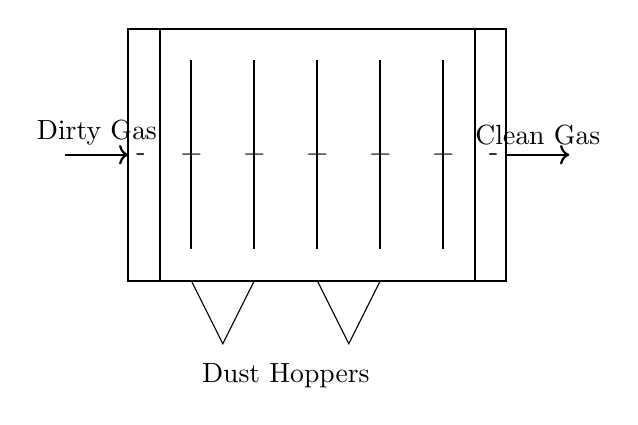
\begin{tikzpicture}[scale=0.8]
        % Box
        \draw[thick] (0,0) rectangle (6,4);
        
        % Discharge electrodes
        \foreach \x in {1,2,3,4,5} {
            \draw[thick] (\x,3.5) -- (\x,0.5);
            \node at (\x,2) {+};
        }
        
        % Collection plates
        \draw[thick] (0.5,0) -- (0.5,4);
        \draw[thick] (5.5,0) -- (5.5,4);
        \node at (0.2, 2) {-};
        \node at (5.8, 2) {-};
        
        % Flow
        \draw[thick, ->] (-1,2) -- (0,2) node[midway, above] {Dirty Gas};
        \draw[thick, ->] (6,2) -- (7,2) node[midway, above] {Clean Gas};
        
        % Hoppers
        \draw (1,0) -- (1.5,-1) -- (2,0);
        \draw (3,0) -- (3.5,-1) -- (4,0);
        \node at (2.5,-1.5) {Dust Hoppers};
    \end{tikzpicture}
    \end{center}

    \begin{itemize}
        \item \textbf{Charging}: Particles acquire electric charge
        \item \textbf{Collection}: Charged particles attracted to plates
        \item \textbf{Efficiency}: 99\% removal of fine particles
    \end{itemize}

    \begin{mnemonicbox}Charge Collect Clean (CCC)\end{mnemonicbox}
\end{solutionbox}

\questionmarks{2}{d}{4}
\textbf{Enlist the types of environmental pollution and give the effects of noise pollution}

\begin{solutionbox}
    \textbf{Environmental pollution types:}
    \begin{itemize}
        \item \textbf{Air pollution}: Atmospheric contamination
        \item \textbf{Water pollution}: Aquatic contamination
        \item \textbf{Soil pollution}: Land contamination
        \item \textbf{Noise pollution}: Sound contamination
    \end{itemize}

    \textbf{Noise Pollution Effects:}
    \begin{itemize}
        \item \textbf{Health effects}: Hearing loss, stress, hypertension
        \item \textbf{Psychological effects}: Irritation, sleep disturbance
        \item \textbf{Performance effects}: Reduced concentration, productivity
        \item \textbf{Communication effects}: Speech interference
    \end{itemize}

    \begin{answertable}{Noise Pollution Impacts}
    \begin{tabulary}{\linewidth}{L L L}
        \toprule
        \textbf{Effect Type} & \textbf{Symptoms} & \textbf{Impact} \\
        \midrule
        \textbf{Physical} & Hearing damage & Permanent loss \\
        \textbf{Mental} & Stress, anxiety & Health issues \\
        \textbf{Social} & Communication problems & Relationship strain \\
        \bottomrule
    \end{tabulary}
    \end{answertable}

    \begin{mnemonicbox}Air Water Soil Sound (AWSS)\end{mnemonicbox}
\end{solutionbox}

\questionmarks{3}{a}{3}
\textbf{What is e-waste? Give effects of e-waste on environment and humans.}

\begin{solutionbox}
    \textbf{E-waste} (Electronic waste) consists of discarded electrical and electronic devices containing hazardous materials.

    \textbf{Environmental Effects:}
    \begin{itemize}
        \item \textbf{Soil contamination}: Heavy metals leaching
        \item \textbf{Water pollution}: Toxic chemical runoff
        \item \textbf{Air pollution}: Burning releases toxic fumes
    \end{itemize}

    \textbf{Human Effects:}
    \begin{itemize}
        \item \textbf{Health hazards}: Lead, mercury poisoning
        \item \textbf{Respiratory problems}: Toxic gas inhalation
        \item \textbf{Skin disorders}: Direct contact with chemicals
    \end{itemize}

    \begin{answertable}{E-waste Hazards}
    \begin{tabulary}{\linewidth}{L L L}
        \toprule
        \textbf{Component} & \textbf{Hazard} & \textbf{Impact} \\
        \midrule
        \textbf{Lead} & Neurotoxin & Brain damage \\
        \textbf{Mercury} & Toxic metal & Kidney damage \\
        \textbf{Cadmium} & Carcinogen & Cancer risk \\
        \bottomrule
    \end{tabulary}
    \end{answertable}

    \begin{mnemonicbox}Electronic Equipment Endangers Everyone (E4)\end{mnemonicbox}
\end{solutionbox}

\questionmarks{3}{a}{3}
\textbf{What is plastic waste? Give effects of plastic waste.}

\begin{solutionbox}
    \textbf{Plastic waste} consists of discarded plastic materials that persist in environment due to non-biodegradable nature.

    \textbf{Effects:}
    \begin{itemize}
        \item \textbf{Marine pollution}: Ocean plastic accumulation
        \item \textbf{Wildlife impact}: Entanglement, ingestion by animals
        \item \textbf{Soil degradation}: Reduced fertility and water infiltration
        \item \textbf{Human health}: Microplastics in food chain
    \end{itemize}

    \textbf{Categories:}
    \begin{itemize}
        \item \textbf{Single-use plastics}: Bags, bottles, straws
        \item \textbf{Packaging waste}: Food containers, wrappings
        \item \textbf{Industrial plastic}: Manufacturing waste
    \end{itemize}

    \begin{mnemonicbox}Plastic Persists, Problems Persist (PPPP)\end{mnemonicbox}
\end{solutionbox}

\questionmarks{3}{b}{3}
\textbf{Give main sources of solid waste.}

\begin{solutionbox}
    \textbf{Solid waste} originates from various human activities and natural processes.

    \textbf{Sources:}
    \begin{itemize}
        \item \textbf{Residential}: Household garbage, food waste
        \item \textbf{Commercial}: Office waste, packaging materials
        \item \textbf{Industrial}: Manufacturing waste, chemicals
        \item \textbf{Agricultural}: Crop residues, animal waste
        \item \textbf{Municipal}: Street sweeping, park maintenance
    \end{itemize}

    \begin{answertable}{Solid Waste Sources}
    \begin{tabulary}{\linewidth}{L L L}
        \toprule
        \textbf{Source} & \textbf{Waste Type} & \textbf{Management} \\
        \midrule
        \textbf{Domestic} & Organic, Plastic & Collection \\
        \textbf{Industrial} & Hazardous, Non-hazardous & Treatment \\
        \textbf{Agricultural} & Biodegradable & Composting \\
        \bottomrule
    \end{tabulary}
    \end{answertable}

    \begin{mnemonicbox}Residential Commercial Industrial Agricultural Municipal (RCIAM)\end{mnemonicbox}
\end{solutionbox}

\questionmarks{3}{b}{3}
\textbf{Enlist various methods of solid waste disposal and explain any one.}

\begin{solutionbox}
    \textbf{Disposal Methods:}
    \begin{itemize}
        \item \textbf{Landfilling}: Controlled waste burial
        \item \textbf{Incineration}: Waste burning with energy recovery
        \item \textbf{Composting}: Organic waste decomposition
        \item \textbf{Recycling}: Material recovery and reuse
    \end{itemize}

    \textbf{Sanitary Landfill:}
    \begin{center}
    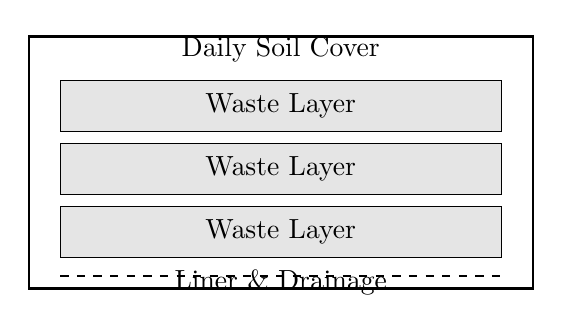
\begin{tikzpicture}[scale=0.8]
        \draw[thick] (0,0) -- (8,0) -- (8,4) -- (0,4) -- cycle;
        \foreach \y in {0.5, 1.5, 2.5} {
            \draw[fill=gray!20] (0.5, \y) rectangle (7.5, \y+0.8);
            \node at (4, \y+0.4) {Waste Layer};
        }
        \draw[dashed] (0.5, 0.2) -- (7.5, 0.2);
        \node at (4, 0.1) {Liner \& Drainage};
        \node at (4, 3.8) {Daily Soil Cover};
    \end{tikzpicture}
    \end{center}

    \begin{itemize}
        \item \textbf{Design}: Engineered system with liners
        \item \textbf{Operation}: Daily cover, compaction
        \item \textbf{Environmental protection}: Leachate and gas control
    \end{itemize}

    \begin{mnemonicbox}Land Incinerate Compost Recycle (LICR)\end{mnemonicbox}
\end{solutionbox}

\questionmarks{3}{c}{4}
\textbf{Explain the working of Liquid Flat Plate Collector with a neat sketch.}

\begin{solutionbox}
    \textbf{Liquid Flat Plate Collector} converts solar radiation into thermal energy for heating water.

    \begin{center}
    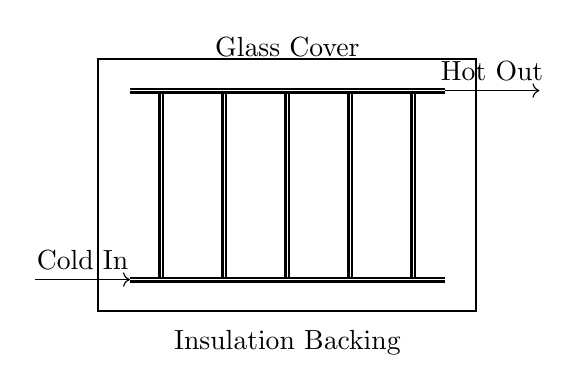
\begin{tikzpicture}[scale=0.8]
        % Frame
        \draw[thick] (0,0) rectangle (6,4);
        % Tubes
        \foreach \x in {1,2,3,4,5} {
            \draw[thick, double] (\x,0.5) -- (\x,3.5);
        }
        % Headers
        \draw[thick, double] (0.5,0.5) -- (5.5,0.5);
        \draw[thick, double] (0.5,3.5) -- (5.5,3.5);
        
        % Labels
        \node at (3,4.2) {Glass Cover};
        \node at (3,-0.5) {Insulation Backing};
        \draw[->] (-1,0.5) -- (0.5,0.5) node[midway, above] {Cold In};
        \draw[->] (5.5,3.5) -- (7,3.5) node[midway, above] {Hot Out};
    \end{tikzpicture}
    \end{center}

    \textbf{Working:}
    \begin{itemize}
        \item \textbf{Solar absorption}: Black absorber plate captures solar energy
        \item \textbf{Heat transfer}: Absorbed heat transfers to flowing liquid
        \item \textbf{Circulation}: Heated liquid rises, cool liquid enters
        \item \textbf{Insulation}: Minimizes heat losses
    \end{itemize}

    \textbf{Components:}
    \begin{itemize}
        \item \textbf{Transparent cover}: Reduces convection losses
        \item \textbf{Absorber plate}: Maximum solar absorption
        \item \textbf{Heat transfer fluid}: Water or antifreeze solution
    \end{itemize}

    \begin{mnemonicbox}Solar Absorption Creates Heat Transfer (SACHT)\end{mnemonicbox}
\end{solutionbox}

\questionmarks{3}{c}{4}
\textbf{Write short note on solar pond}

\begin{solutionbox}
    \textbf{Solar pond} is a pool of saltwater that acts as both solar collector and thermal storage system.

    \textbf{Structure:}
    \begin{itemize}
        \item \textbf{Upper zone}: Low salt concentration
        \item \textbf{Middle zone}: Increasing salt gradient
        \item \textbf{Lower zone}: High salt concentration
    \end{itemize}

    \textbf{Working:}
    \begin{itemize}
        \item \textbf{Density gradient}: Prevents convection mixing
        \item \textbf{Heat storage}: Bottom layer stores thermal energy
        \item \textbf{Temperature}: Can reach 70-85$^{\circ}$C at bottom
    \end{itemize}

    \textbf{Applications:}
    \begin{itemize}
        \item \textbf{Power generation}: Steam production
        \item \textbf{Industrial heating}: Process heat supply
        \item \textbf{Desalination}: Water purification
    \end{itemize}

    \begin{mnemonicbox}Salt Stores Solar Thermal (SSST)\end{mnemonicbox}
\end{solutionbox}

\questionmarks{3}{d}{4}
\textbf{Explain Savonious wind mill with a neat sketch.}

\begin{solutionbox}
    \textbf{Savonius wind turbine} is a vertical axis wind turbine with S-shaped rotor blades.

    \begin{center}
    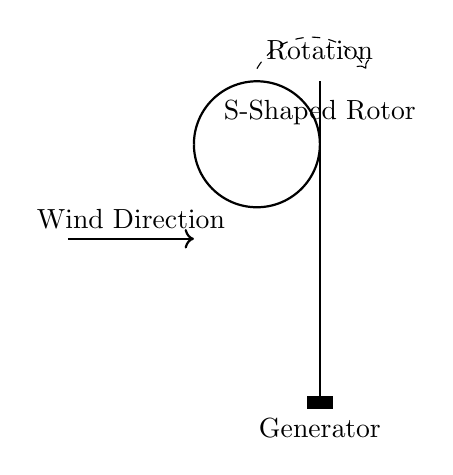
\begin{tikzpicture}[scale=0.8]
        % Axis
        \draw[thick] (4,0) -- (4,5);
        \node at (4,-0.5) {Generator};
        \draw[fill=black] (3.8,-0.2) rectangle (4.2,0);
        
        % S-Rotor (Top view projection)
        \draw[thick] (2,4) arc (180:360:1);
        \draw[thick] (4,4) arc (0:180:1);
        \node at (4, 4.5) {S-Shaped Rotor};
        
        % Wind
        \draw[thick, ->] (0,2.5) -- (2,2.5) node[midway, above] {Wind Direction};
        
        % Rotation
        \draw[->, dashed] (3, 5.2) arc (150:30:1);
        \node at (4, 5.5) {Rotation};
    \end{tikzpicture}
    \end{center}

    \textbf{Working:}
    \begin{itemize}
        \item \textbf{Drag principle}: Wind creates differential drag on blades
        \item \textbf{Rotation}: S-shape causes continuous rotation
        \item \textbf{Self-starting}: Starts at low wind speeds
        \item \textbf{Vertical axis}: Independent of wind direction
    \end{itemize}

    \textbf{Advantages:}
    \begin{itemize}
        \item \textbf{Simple design}: Low maintenance requirements
        \item \textbf{Low noise}: Quiet operation
        \item \textbf{All wind directions}: Omnidirectional capability
    \end{itemize}

    \textbf{Disadvantages:}
    \begin{itemize}
        \item \textbf{Lower efficiency}: 20-30\% compared to HAWT
        \item \textbf{Space requirement}: Larger area needed
    \end{itemize}

    \begin{mnemonicbox}S-Shape Starts Slowly (SSS)\end{mnemonicbox}
\end{solutionbox}

\questionmarks{3}{d}{4}
\textbf{Give the comparison between Horizontal Axis and Vertical Axis wind mills.}

\begin{solutionbox}
    Wind turbines are classified based on rotor axis orientation.

    \begin{answertable}{HAWT vs VAWT Comparison}
    \begin{tabulary}{\linewidth}{L L L}
        \toprule
        \textbf{Parameter} & \textbf{Horizontal Axis (HAWT)} & \textbf{Vertical Axis (VAWT)} \\
        \midrule
        \textbf{Efficiency} & 35-45\% & 20-30\% \\
        \textbf{Wind direction} & Must face wind & Any direction \\
        \textbf{Installation} & Tower required & Ground level possible \\
        \textbf{Maintenance} & Difficult access & Easy access \\
        \textbf{Noise} & Higher & Lower \\
        \textbf{Cost} & Higher & Lower \\
        \bottomrule
    \end{tabulary}
    \end{answertable}

    \textbf{HAWT Features:}
    \begin{itemize}
        \item \textbf{Upwind design}: Rotor faces wind
        \item \textbf{Pitch control}: Blade angle adjustment
        \item \textbf{Yaw system}: Wind direction tracking
    \end{itemize}

    \textbf{VAWT Features:}
    \begin{itemize}
        \item \textbf{Omnidirectional}: No wind tracking needed
        \item \textbf{Ground installation}: Easier maintenance
        \item \textbf{Lower wind speeds}: Better performance
    \end{itemize}

    \begin{mnemonicbox}Horizontal High, Vertical Versatile (HHVV)\end{mnemonicbox}
\end{solutionbox}

\questionmarks{4}{a}{3}
\textbf{Give effects of climate change.}

\begin{solutionbox}
    \textbf{Climate change} causes widespread environmental and socio-economic impacts globally.

    \textbf{Environmental Effects:}
    \begin{itemize}
        \item \textbf{Temperature rise}: Global average increase
        \item \textbf{Sea level rise}: Thermal expansion and ice melting
        \item \textbf{Weather extremes}: Intense storms, droughts, floods
        \item \textbf{Ecosystem shifts}: Species migration and extinction
    \end{itemize}

    \textbf{Socio-economic Effects:}
    \begin{itemize}
        \item \textbf{Agricultural impact}: Crop yield changes
        \item \textbf{Water resources}: Availability and quality issues
        \item \textbf{Human health}: Heat stress, disease spread
        \item \textbf{Economic losses}: Infrastructure damage
    \end{itemize}

    \begin{answertable}{Climate Change Impacts}
    \begin{tabulary}{\linewidth}{L L L}
        \toprule
        \textbf{Impact Category} & \textbf{Examples} & \textbf{Severity} \\
        \midrule
        \textbf{Environmental} & Melting glaciers & High \\
        \textbf{Agricultural} & Crop failure & Medium \\
        \textbf{Health} & Heat waves & High \\
        \bottomrule
    \end{tabulary}
    \end{answertable}

    \begin{mnemonicbox}Temperature Sea Weather Ecosystem (TSWE)\end{mnemonicbox}
\end{solutionbox}

\questionmarks{4}{a}{3}
\textbf{Write a short note on Green House gases.}

\begin{solutionbox}
    \textbf{Greenhouse gases} trap heat in Earth's atmosphere, causing global warming through greenhouse effect.

    \textbf{Major Greenhouse Gases:}
    \begin{itemize}
        \item \textbf{Carbon dioxide (CO\textsubscript{2})}: 76\% of emissions
        \item \textbf{Methane (CH\textsubscript{4})}: 16\% of emissions
        \item \textbf{Nitrous oxide (N\textsubscript{2}O)}: 6\% of emissions
        \item \textbf{Fluorinated gases}: 2\% of emissions
    \end{itemize}

    \textbf{Sources:}
    \begin{itemize}
        \item \textbf{CO\textsubscript{2}}: Fossil fuel burning, deforestation
        \item \textbf{CH\textsubscript{4}}: Agriculture, landfills, livestock
        \item \textbf{N\textsubscript{2}O}: Fertilizers, fossil fuel combustion
    \end{itemize}

    \textbf{Global Warming Potential:}
    \begin{itemize}
        \item \textbf{CO\textsubscript{2}}: Reference (GWP = 1)
        \item \textbf{CH\textsubscript{4}}: 25 times CO\textsubscript{2}
        \item \textbf{N\textsubscript{2}O}: 298 times CO\textsubscript{2}
    \end{itemize}

    \begin{mnemonicbox}Carbon Methane Nitrous Fluorine (CMNF)\end{mnemonicbox}
\end{solutionbox}

\questionmarks{4}{b}{4}
\textbf{Explain climate change Management.}

\begin{solutionbox}
    \textbf{Climate change management} involves strategies to reduce greenhouse gas emissions and adapt to climate impacts.

    \textbf{Mitigation Strategies:}
    \begin{itemize}
        \item \textbf{Renewable energy}: Solar, wind, hydroelectric power
        \item \textbf{Energy efficiency}: Improved building designs, LED lighting
        \item \textbf{Carbon sequestration}: Forest conservation, tree planting
        \item \textbf{Sustainable transport}: Electric vehicles, public transport
    \end{itemize}

    \textbf{Adaptation Strategies:}
    \begin{itemize}
        \item \textbf{Infrastructure resilience}: Flood defenses, drought-resistant crops
        \item \textbf{Water management}: Rainwater harvesting, efficient irrigation
        \item \textbf{Coastal protection}: Sea walls, mangrove restoration
        \item \textbf{Emergency preparedness}: Early warning systems
    \end{itemize}

    \textbf{Policy Measures:}
    \begin{itemize}
        \item \textbf{Carbon pricing}: Tax on emissions
        \item \textbf{Renewable energy targets}: Clean energy goals
        \item \textbf{Building codes}: Energy efficiency standards
    \end{itemize}

    \begin{mnemonicbox}Mitigation Adaptation Policy (MAP)\end{mnemonicbox}
\end{solutionbox}

\questionmarks{4}{b}{4}
\textbf{Give effects of ozone layer depletion.}

\begin{solutionbox}
    \textbf{Ozone layer depletion} reduces stratospheric ozone, allowing harmful UV radiation to reach Earth.

    \textbf{Effects on Humans:}
    \begin{itemize}
        \item \textbf{Skin cancer}: Increased UV-B radiation exposure
        \item \textbf{Eye cataracts}: UV damage to eye lens
        \item \textbf{Immune suppression}: Weakened immune system
        \item \textbf{Premature aging}: Skin damage acceleration
    \end{itemize}

    \textbf{Effects on Environment:}
    \begin{itemize}
        \item \textbf{Crop damage}: Reduced agricultural productivity
        \item \textbf{Marine ecosystem}: Phytoplankton reduction
        \item \textbf{Material degradation}: Plastic and rubber damage
        \item \textbf{Climate change}: Ozone as greenhouse gas
    \end{itemize}

    \begin{answertable}{UV Radiation Effects}
    \begin{tabulary}{\linewidth}{L L L}
        \toprule
        \textbf{UV Type} & \textbf{Wavelength} & \textbf{Effect} \\
        \midrule
        \textbf{UV-A} & 320-400 nm & Skin aging \\
        \textbf{UV-B} & 280-320 nm & Sunburn, cancer \\
        \textbf{UV-C} & 200-280 nm & Blocked by ozone \\
        \bottomrule
    \end{tabulary}
    \end{answertable}

    \begin{mnemonicbox}Skin Eyes Immunity Climate (SEIC)\end{mnemonicbox}
\end{solutionbox}

\questionmarks{4}{c}{7}
\textbf{Explain biogas plant with sketch.}

\begin{solutionbox}
    \textbf{Biogas plant} produces methane-rich gas through anaerobic digestion of organic waste.

    \begin{center}
    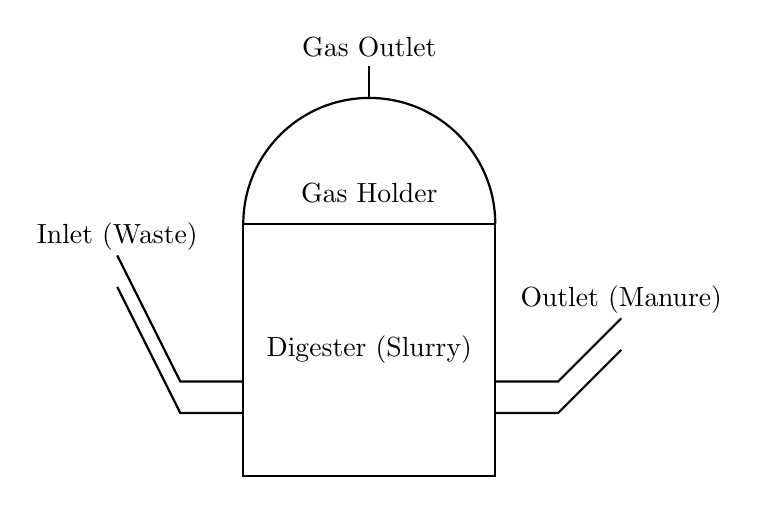
\begin{tikzpicture}[scale=0.8]
        % Tank
        \draw[thick] (2,0) rectangle (6,4);
        \node at (4,2) {Digester (Slurry)};
        
        % Dome
        \draw[thick] (2,4) arc (180:0:2);
        \node at (4,4.5) {Gas Holder};
        \draw[thick] (4,6) -- (4,6.5) node[above] {Gas Outlet};
        
        % Inlet
        \draw[thick] (0,3) -- (1,1) -- (2,1);
        \draw[thick] (0,3.5) -- (1,1.5) -- (2,1.5);
        \node at (0,3.8) {Inlet (Waste)};
        
        % Outlet
        \draw[thick] (6,1) -- (7,1) -- (8,2);
        \draw[thick] (6,1.5) -- (7,1.5) -- (8,2.5);
        \node at (8,2.8) {Outlet (Manure)};
    \end{tikzpicture}
    \end{center}

    \textbf{Components:}
    \begin{itemize}
        \item \textbf{Digester tank}: Anaerobic fermentation chamber
        \item \textbf{Gas dome}: Biogas collection and storage
        \item \textbf{Inlet pipe}: Waste material feeding
        \item \textbf{Outlet pipe}: Digested slurry removal
    \end{itemize}

    \textbf{Process:}
    \begin{itemize}
        \item \textbf{Hydrolysis}: Complex organics break down
        \item \textbf{Acidogenesis}: Acid-forming bacteria action
        \item \textbf{Methanogenesis}: Methane-producing bacteria
        \item \textbf{Gas production}: 50-70\% methane, 30-40\% CO\textsubscript{2}
    \end{itemize}

    \textbf{Operating Conditions:}
    \begin{itemize}
        \item \textbf{Temperature}: 30-40{\circ} optimal
        \item \textbf{pH}: 6.8-7.2 range
        \item \textbf{Retention time}: 15-30 days
        \item \textbf{C:N ratio}: 20-30:1 optimal
    \end{itemize}

    \textbf{Applications:}
    \begin{itemize}
        \item \textbf{Cooking fuel}: Household energy needs
        \item \textbf{Lighting}: Gas lamp illumination
        \item \textbf{Electricity}: Generator power
        \item \textbf{Fertilizer}: Nutrient-rich slurry
    \end{itemize}

    \textbf{Advantages:}
    \begin{itemize}
        \item \textbf{Renewable energy}: Sustainable fuel source
        \item \textbf{Waste management}: Organic waste utilization
        \item \textbf{Environmental benefits}: Reduced methane emissions
        \item \textbf{Economic benefits}: Cost savings on fuel
    \end{itemize}

    \begin{mnemonicbox}Biogas Benefits: Renewable Waste Environment Economy (BRWEE)\end{mnemonicbox}
\end{solutionbox}

\questionmarks{5}{a}{4}
\textbf{Write short note on global warming.}

\begin{solutionbox}
    \textbf{Global warming} refers to long-term increase in Earth's average surface temperature due to human activities.

    \textbf{Causes:}
    \begin{itemize}
        \item \textbf{Greenhouse gases}: CO\textsubscript{2}, CH\textsubscript{4}, N\textsubscript{2}O emissions
        \item \textbf{Deforestation}: Reduced carbon absorption
        \item \textbf{Industrial activities}: Fossil fuel combustion
        \item \textbf{Transportation}: Vehicle emissions
    \end{itemize}

    \textbf{Effects:}
    \begin{itemize}
        \item \textbf{Temperature rise}: 1.1{\circ} since pre-industrial times
        \item \textbf{Ice melting}: Arctic sea ice, glaciers shrinking
        \item \textbf{Sea level rise}: Coastal flooding threat
        \item \textbf{Weather changes}: Extreme events frequency
    \end{itemize}

    \textbf{Evidence:}
    \begin{itemize}
        \item \textbf{Temperature records}: Warmest years in recent decades
        \item \textbf{Ice core data}: Historical CO\textsubscript{2} levels
        \item \textbf{Satellite measurements}: Global temperature monitoring
    \end{itemize}

    \textbf{Solutions:}
    \begin{itemize}
        \item \textbf{Renewable energy}: Clean power sources
        \item \textbf{Energy efficiency}: Reduced consumption
        \item \textbf{Carbon capture}: Technology development
        \item \textbf{International cooperation}: Paris Agreement
    \end{itemize}

    \begin{mnemonicbox}Greenhouse Gases Generate Global Change (GGGC)\end{mnemonicbox}
\end{solutionbox}

\questionmarks{5}{b}{4}
\textbf{Explain 5R concept.}

\begin{solutionbox}
    \textbf{5R concept} is waste management hierarchy for sustainable resource utilization.

    \begin{center}
    \begin{tikzpicture}[node distance=1.5cm, auto]
        \node (root) [gtu block] {5R Hierarchy};
        \node (r1) [gtu block, below=of root] {Refuse};
        \node (r2) [gtu block, below=of r1] {Reduce};
        \node (r3) [gtu block, below=of r2] {Reuse};
        \node (r4) [gtu block, below=of r3] {Repurpose};
        \node (r5) [gtu block, below=of r4] {Recycle};

        \draw [gtu arrow] (root) -- (r1);
        \draw [gtu arrow] (r1) -- (r2);
        \draw [gtu arrow] (r2) -- (r3);
        \draw [gtu arrow] (r3) -- (r4);
        \draw [gtu arrow] (r4) -- (r5);
    \end{tikzpicture}
    \end{center}

    \textbf{The 5 R's:}

    \textbf{1. Refuse:}
    \begin{itemize}
        \item \textbf{Avoid unnecessary items}: Say no to single-use products
        \item \textbf{Examples}: Plastic bags, straws, excessive packaging
    \end{itemize}

    \textbf{2. Reduce:}
    \begin{itemize}
        \item \textbf{Minimize consumption}: Use less resources
        \item \textbf{Examples}: Energy conservation, water saving
    \end{itemize}

    \textbf{3. Reuse:}
    \begin{itemize}
        \item \textbf{Multiple use}: Extend product life
        \item \textbf{Examples}: Glass jars as containers, paper both sides
    \end{itemize}

    \textbf{4. Repurpose:}
    \begin{itemize}
        \item \textbf{Creative reuse}: New function for old items
        \item \textbf{Examples}: Tire planters, bottle bird feeders
    \end{itemize}

    \textbf{5. Recycle:}
    \begin{itemize}
        \item \textbf{Material recovery}: Process into new products
        \item \textbf{Examples}: Paper, plastic, metal recycling
    \end{itemize}

    \textbf{Benefits:}
    \begin{itemize}
        \item \textbf{Waste reduction}: Less landfill burden
        \item \textbf{Resource conservation}: Natural resource preservation
        \item \textbf{Cost savings}: Economic benefits
        \item \textbf{Environmental protection}: Pollution reduction
    \end{itemize}

    \begin{mnemonicbox}Refuse Reduce Reuse Repurpose Recycle (R5)\end{mnemonicbox}
\end{solutionbox}

\questionmarks{5}{c}{3}
\textbf{Explain the benefits of Green building.}

\begin{solutionbox}
    \textbf{Green building} incorporates sustainable design and construction practices for environmental and human benefits.

    \textbf{Environmental Benefits:}
    \begin{itemize}
        \item \textbf{Energy efficiency}: Reduced power consumption
        \item \textbf{Water conservation}: Efficient water systems
        \item \textbf{Waste reduction}: Construction and operational waste minimization
    \end{itemize}

    \textbf{Economic Benefits:}
    \begin{itemize}
        \item \textbf{Operating cost savings}: Lower utility bills
        \item \textbf{Increased property value}: Market premium
        \item \textbf{Tax incentives}: Government rebates
    \end{itemize}

    \textbf{Health Benefits:}
    \begin{itemize}
        \item \textbf{Indoor air quality}: Better ventilation systems
        \item \textbf{Natural lighting}: Improved occupant comfort
        \item \textbf{Toxic material reduction}: Healthier environment
    \end{itemize}

    \begin{answertable}{Green Building Impacts}
    \begin{tabulary}{\linewidth}{L L L}
        \toprule
        \textbf{Benefit Type} & \textbf{Examples} & \textbf{Impact} \\
        \midrule
        \textbf{Environmental} & Energy saving & 30-50\% reduction \\
        \textbf{Economic} & Cost savings & 20\% operating costs \\
        \textbf{Health} & Air quality & Productivity increase \\
        \bottomrule
    \end{tabulary}
    \end{answertable}

    \begin{mnemonicbox}Green Buildings Give Environmental Economic Health (GBEEH)\end{mnemonicbox}
\end{solutionbox}

\questionmarks{5}{d}{3}
\textbf{Enlist various Acts related to environment in India and explain any one.}

\begin{solutionbox}
    \textbf{Environmental Acts in India:}
    \begin{itemize}
        \item \textbf{Water (Prevention and Control of Pollution) Act, 1974}
        \item \textbf{Air (Prevention and Control of Pollution) Act, 1981}
        \item \textbf{Environment Protection Act, 1986}
        \item \textbf{Wildlife Protection Act, 1972}
        \item \textbf{Forest (Conservation) Act, 1980}
        \item \textbf{Biodiversity Act, 2002}
    \end{itemize}

    \textbf{Environment Protection Act, 1986:}
    
    \textbf{Objectives:}
    \begin{itemize}
        \item \textbf{Comprehensive framework}: Overall environmental protection
        \item \textbf{Pollution prevention}: Air, water, soil contamination control
        \item \textbf{Standard setting}: Environmental quality standards
        \item \textbf{Enforcement}: Penalties for violations
    \end{itemize}

    \textbf{Powers:}
    \begin{itemize}
        \item \textbf{Central government authority}: Environmental regulations
        \item \textbf{Inspection rights}: Industrial facilities monitoring
        \item \textbf{Closure orders}: Non-compliant industries
        \item \textbf{Emergency measures}: Environmental hazards response
    \end{itemize}

    \textbf{Significance:}
    \begin{itemize}
        \item \textbf{Umbrella legislation}: Covers all environmental aspects
        \item \textbf{Post-Bhopal disaster}: Response to industrial accidents
    \end{itemize}

    \begin{mnemonicbox}Water Air Environment Wildlife Forest Biodiversity (WAEWFB)\end{mnemonicbox}
\end{solutionbox}

\end{document}
